% !TEX root = ../thesis-example.tex
%
\chapter{Resultados}
\label{Resultados}

En este capítulo se presentan los resultados de la implementación de la metodología presentada en el Capítulo \ref{Metodologia}. 
Los algoritmos fueron implementados en Mathematica y Matlab, además fueron aplicados sobre las bases de datos de mercados financieros como se ha descrito en la Sección \ref{sec_data}.
En las siguientes secciones presentaremos los resultados de la estimación de mínimos de entropía así como la optimización de los parámetros libres del algoritmo.


\section{Resultado del cálculo de entropías simple}
{
La primera etapa de este estudio consistió en aplicar el algoritmo descrito en la Sección \ref{sec_algorithm}.
En este caso se calculó la entropía sobre los cuatro mercados analizados. 

En la Figura \ref{precioseps} se tienen los precios en el mercado y su evolución en el tiempo, tal como se muestran dichos precios no se les ha aplicado ningún filtro de media móvil ni ninguna suavización de la curva.
El único proceso aplicado a los datos en esta etapa corresponde a la depuración de datos corruptos.

\begin{figure}[h!]
	\centering
	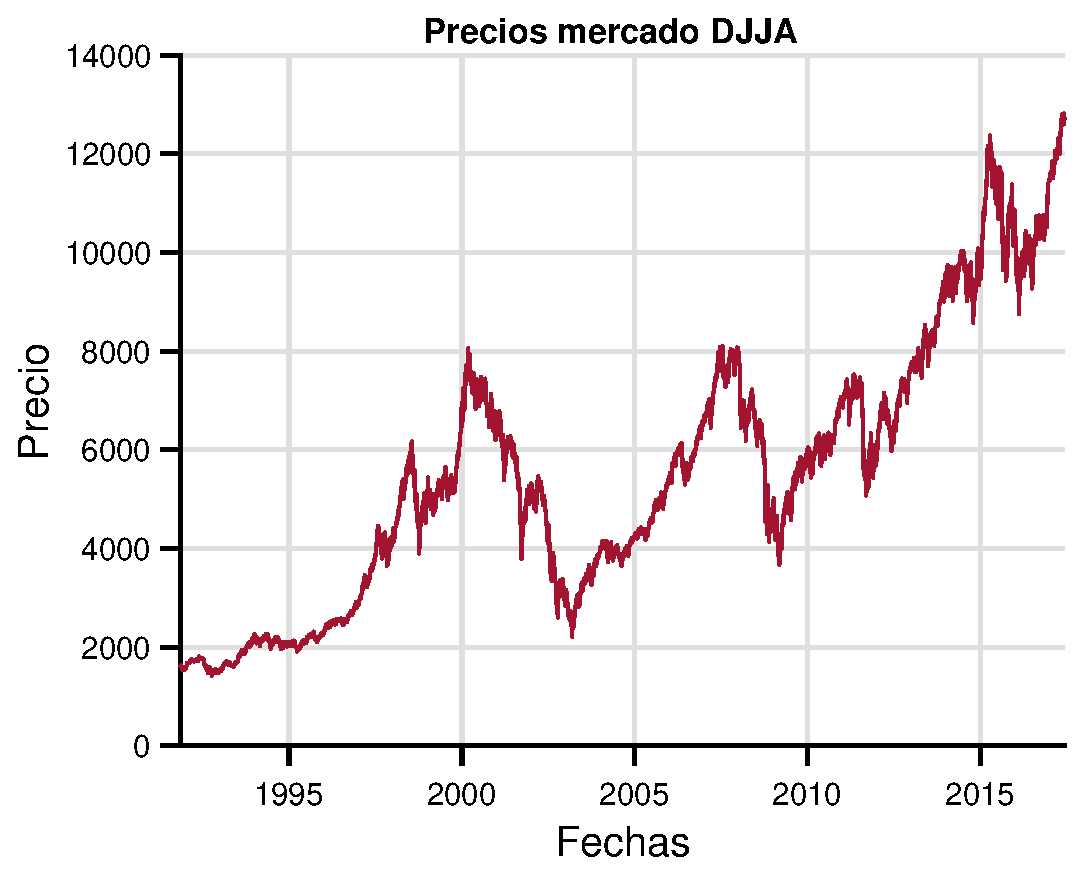
\includegraphics[width=0.7\linewidth]{figures/precioseps}
	\caption{Evolución temporal de los precios en el mercado DJJA.}
	\label{precioseps}
\end{figure}

A partir de los datos depurados y ordenados se calcularon lo retornos como se explica en la sección \ref{Metodologia}. Se aplicó el algoritmo de la Figura \ref{diagramaentropia1}. 
En la figura \ref{onlyreturnseps} se aprecia que los retornos fluctúan entorno a una media de valor cero. 
Sin embargo se aprecia que existen mínimos en el valor del retorno, como es el caso del segundo mínimo, que además es el mínimo global de todos los retornos (18-Jan-2008).

\begin{figure}[h!]
	\centering
	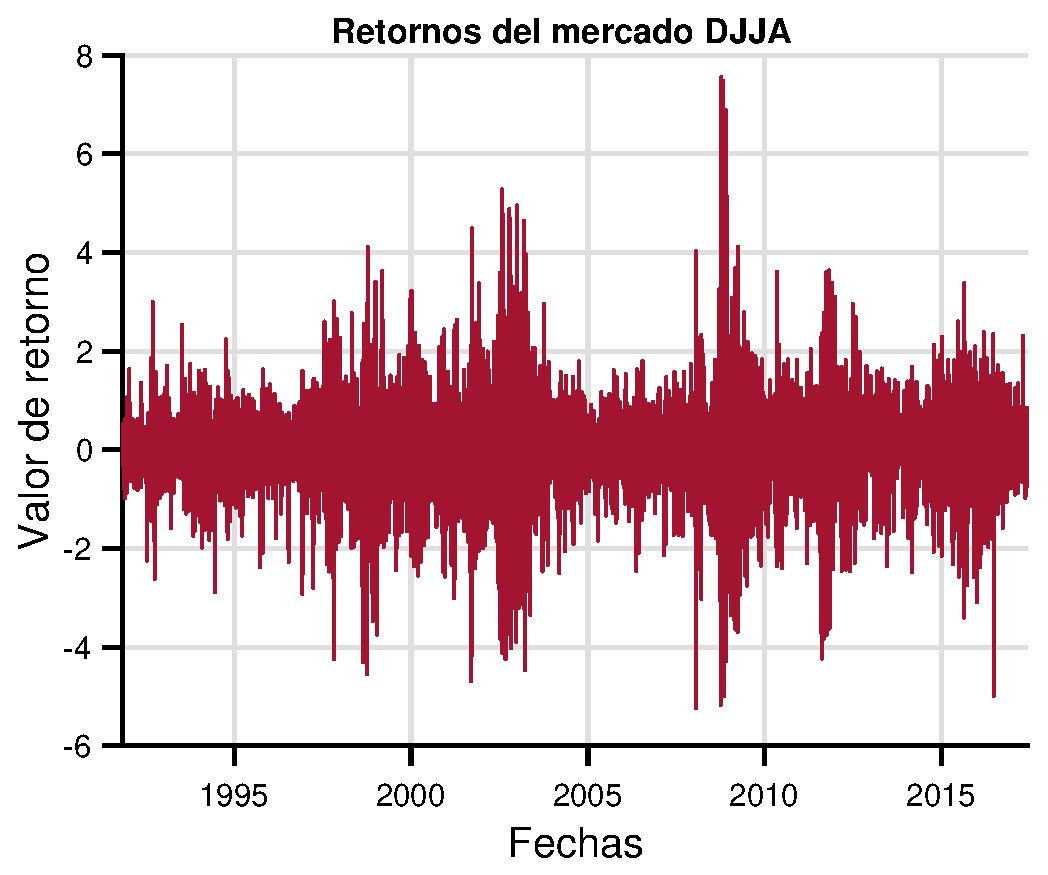
\includegraphics[width=0.7\linewidth]{figures/onlyreturnseps}
	\caption{Retornos para el mercado DJJA.}
	\label{onlyreturnseps}
\end{figure}

Posteriormente se procedió a calcular la entropía de los mercados financieros aplicando el algoritmo descrito en la Sección \ref{sec_entropia}.
\begin{figure}[h!]
	\centering
	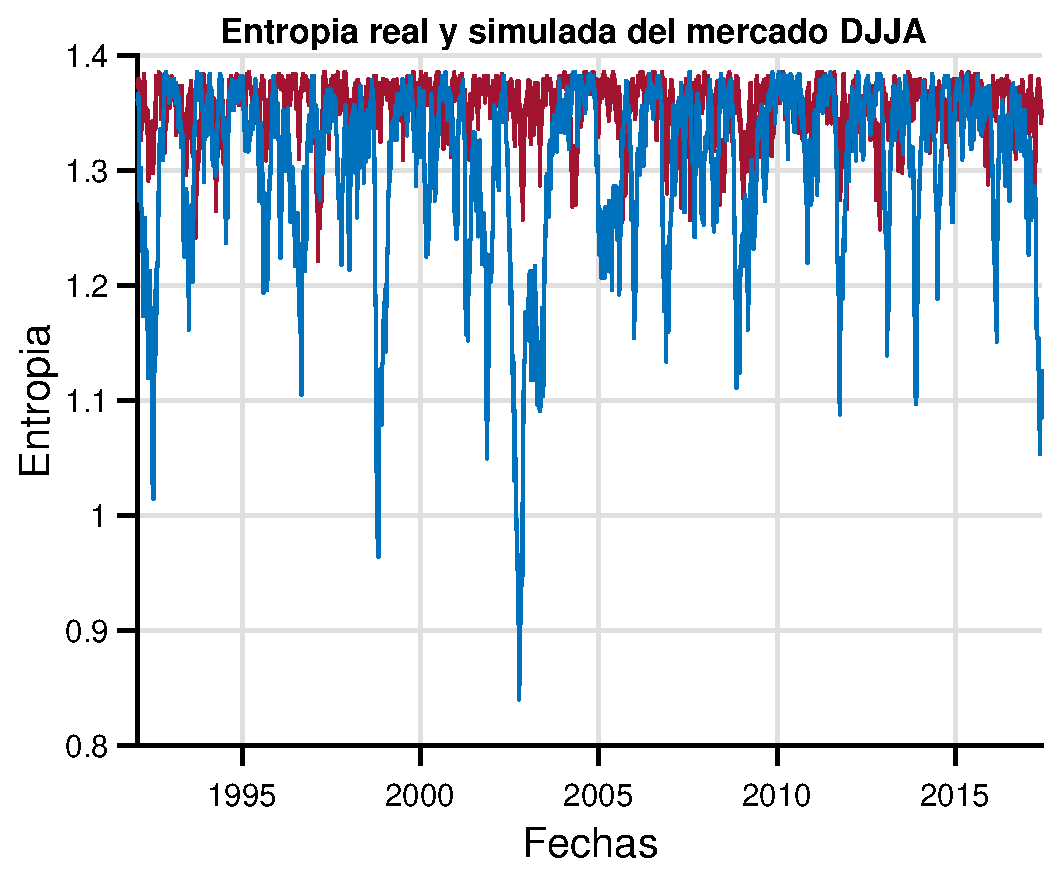
\includegraphics[width=12cm]{figures/onlyentropyeps}
	\caption{Entropía para un mercado simulado y un mercado eficiente. Mercado real DJJA (línea azul) y mercado eficiente DJJA (línea roja).}
	\label{onlyentropyeps}
\end{figure}
En la figura \ref{onlyentropyeps} se presentan los resultados del calculo de entropia con una ventana deslizante de 50 dias	.
Se observa que la entropía posee valores mínimos en la misma fecha (18-Jan-2008) del segundo mínimo que muestra el gráfico de los precios (Ver Figura \ref{precioseps}). 
Sin embargo, el minimo de entropia mas significativo se observa el 29-Jul-2002.
Un mínimo es observado cuando varias fechas consecutivas el precio es más bajo, resultando el valor de retorno negativo. 


}

\section{Resultado del cálculo de entropías con medias móviles}
Se aplico el metodo descerito en la Seccion \ref{metodo_MAV}.
Al aplicar ventanas deslizantes se observa qur el intervalo de la ventana impacta directamente la curva de precios.
De este modo se observa que una ventana deslizante grande (e.g. 50 dias, ver  Figura \ref{mav10Entropy10nq23}) tiene un efecto de suavizado de la curva mas claro que una ventana corta (e.g., 10 dias, ver Figura \ref{mav10Entropy10nq23}) lo que permite observar una cantidad diferente de picos en los valores mínimos de entropía en ambos casos. 



\begin{figure}[h!]
	\centering
	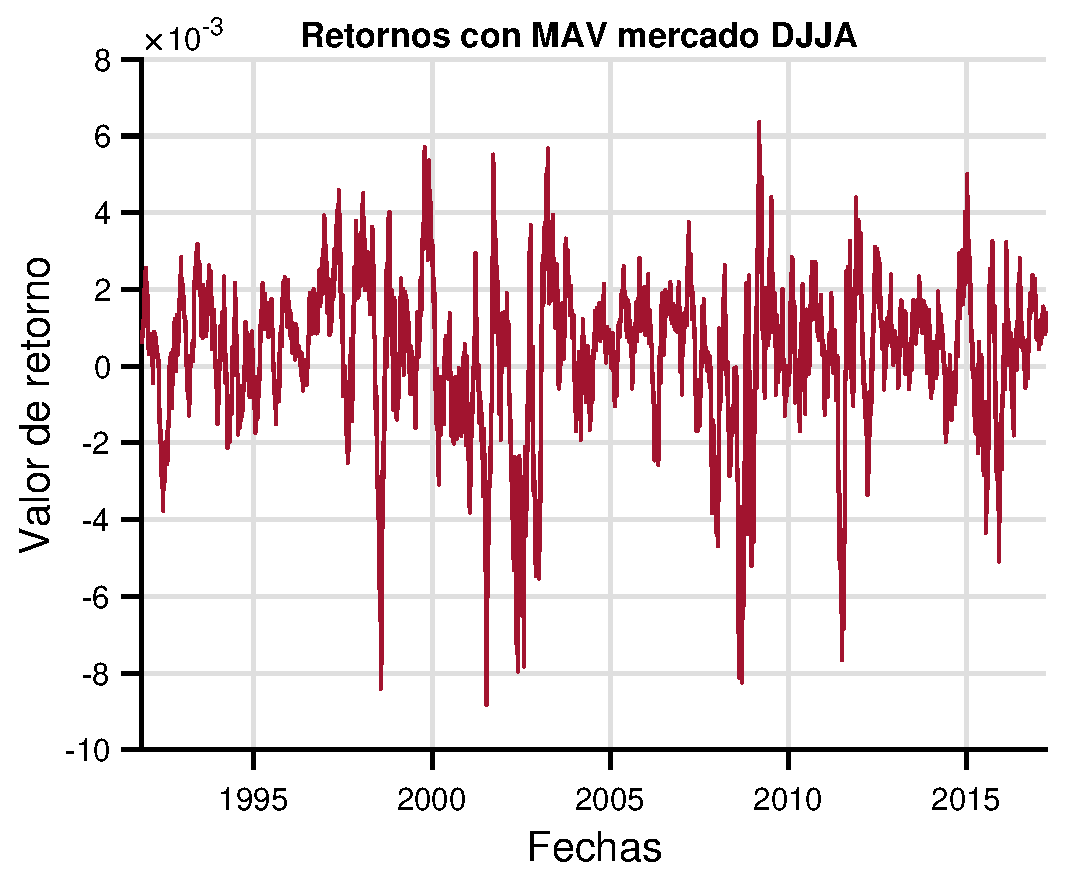
\includegraphics[width=12cm]{figures/MAVreturnseps}
	\caption{Retornos con una media móvil de 50 días aplicada para el mercado DJJA.}
	\label{fig:mavreturnseps}
\end{figure}

En la gráfica \ref{fig:mavreturnseps} se puede apreciar que la representación de los datos es menos conglomerada debido a que se aplicó una ventana de 50 días. Este filtrado de datos permite que la gráfica conserve su comportamiento pero que sea fácil identificar puntos de interés.



\begin{figure}[h!]
	\centering
	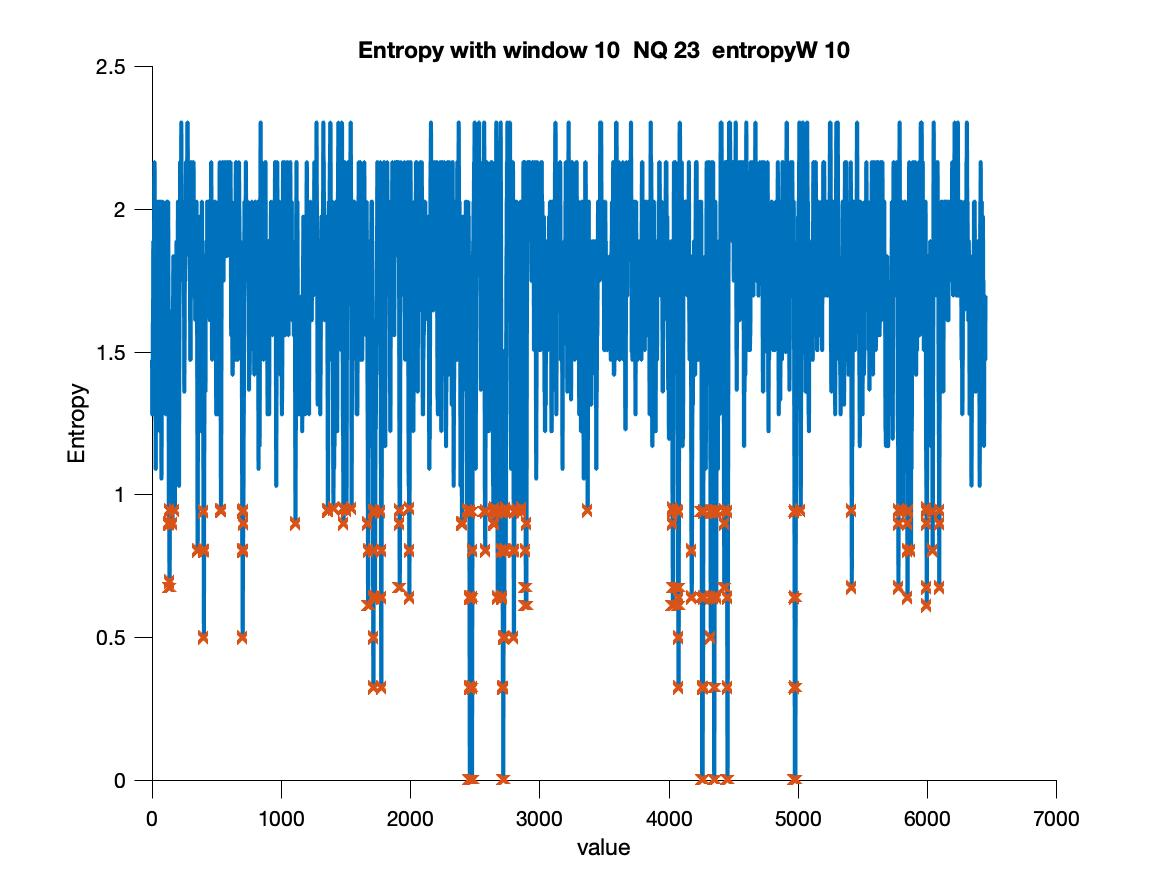
\includegraphics[width=12cm]{figures_matlab/Entropy_window_10_NQ_23_entropyW_10.jpg}
		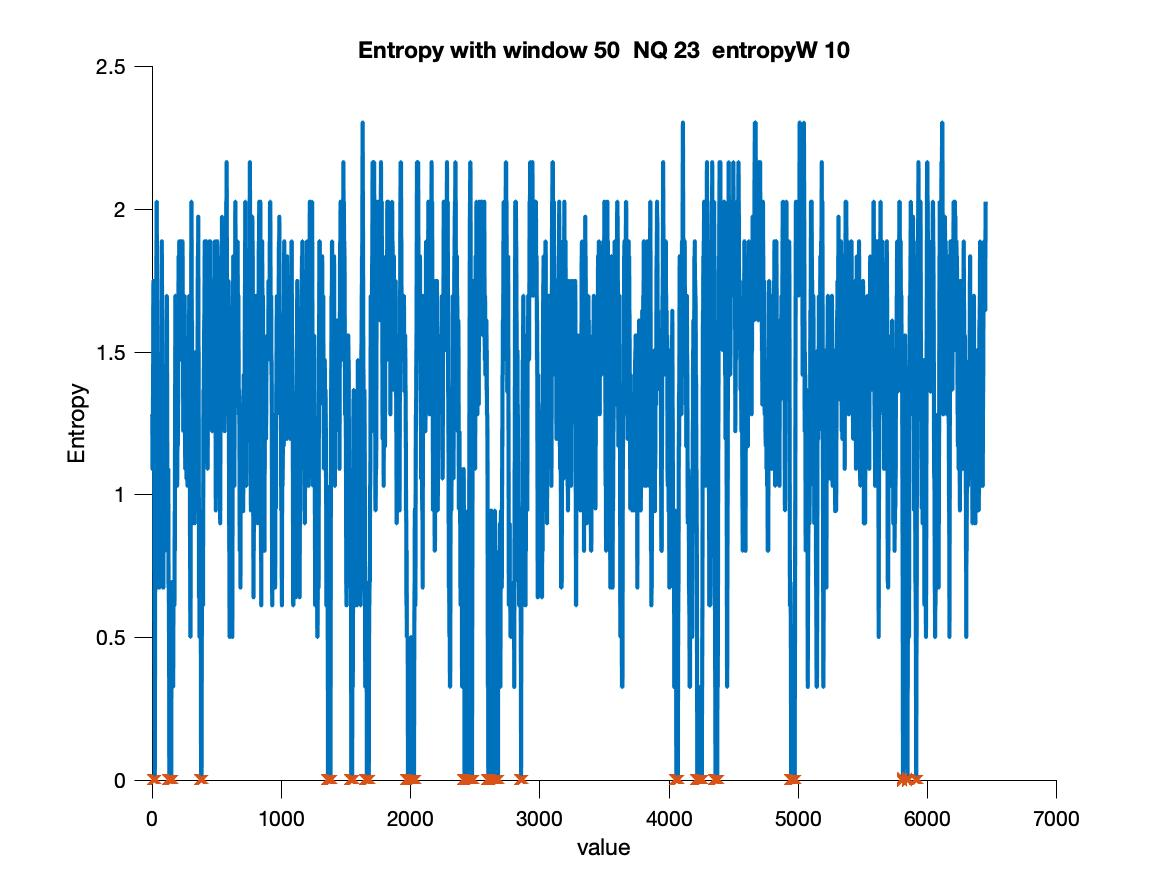
\includegraphics[width=12cm]{figures_matlab/Entropy_window_50_NQ_23_entropyW_10.jpg}
	\caption{Arriba: Valores de entropía con filtro de media móvil de 10 días y agrupación de 10 en 10 para la entropía de Shannon en el caso de 23 cuantiles el mercado DJJA.
	Abajo:Valores de entropía con filtro de media móvil de 50 días y agrupación de 10 en 10 para la entropía de Shannon en el caso de 23 cuantiles el mercado DJJA.}
	\label{mav10Entropy10nq23}
\end{figure}


\section{Búsqueda de mínimos de entropía}

Este metodo se aplico N veces con un intervalo de ventanas deslizantes de 10 a 50,  numero de cuantiles de 4 hasta 130 y ventana glisante de calculo de entropia de 10 a 200.


A partir de este resultado se puede generar un heat map de minimos de entropia y su respectiva senal a ruido SNR, ver Figura 4.3. 
Este heatmap facilita la visualizacion de minimos de entropia para cada valor de nq, w, dt se puede observar en la figura \ref{all_entropy}.



Por ejemplo: 
Entonces es cuando con base en un "heat map" se elige para una ventana de entropía de 10 en 10 con 133 cuantiles y que arroja más de 110 mínimos de entropía. Ello se puede ver en la Figura \ref{caso1}. 


\begin{figure}[h]
	\centering
	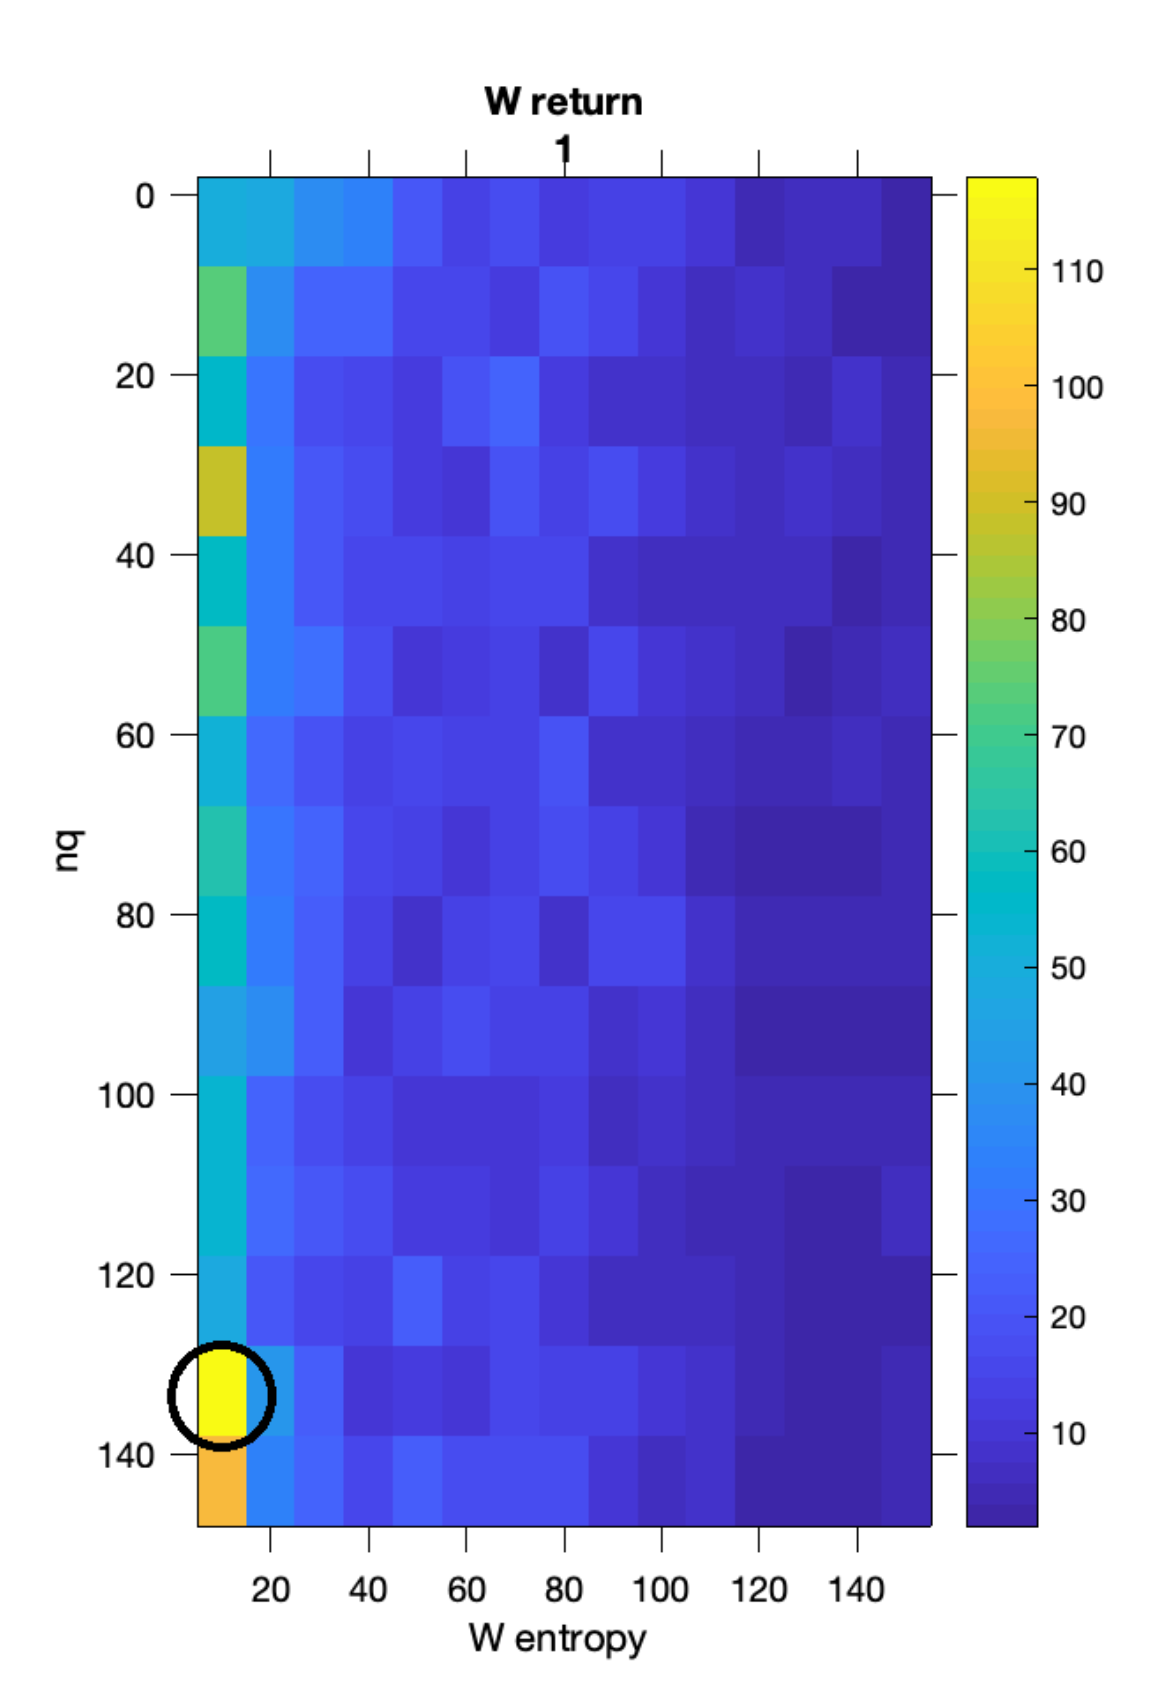
\includegraphics[width=0.7\linewidth]{figures/ejemplo_min_entropy}
	\caption{Cantidades de mínimos de entropía. Caso de estudio para 123 cuantiles y una ventana para la entropía con valor 10.}
	\label{caso1}
\end{figure}

De esos mínimos de entropía se debe hacer una selección de valores que realmente son mínimos de entropía y que no son solo ruido. Del mismo modo con un "heat map" se estudia la señal a ruido de esa misma región como se muestra en la Figura \ref{caso1SNR} .

\begin{figure}[h]
	\centering
	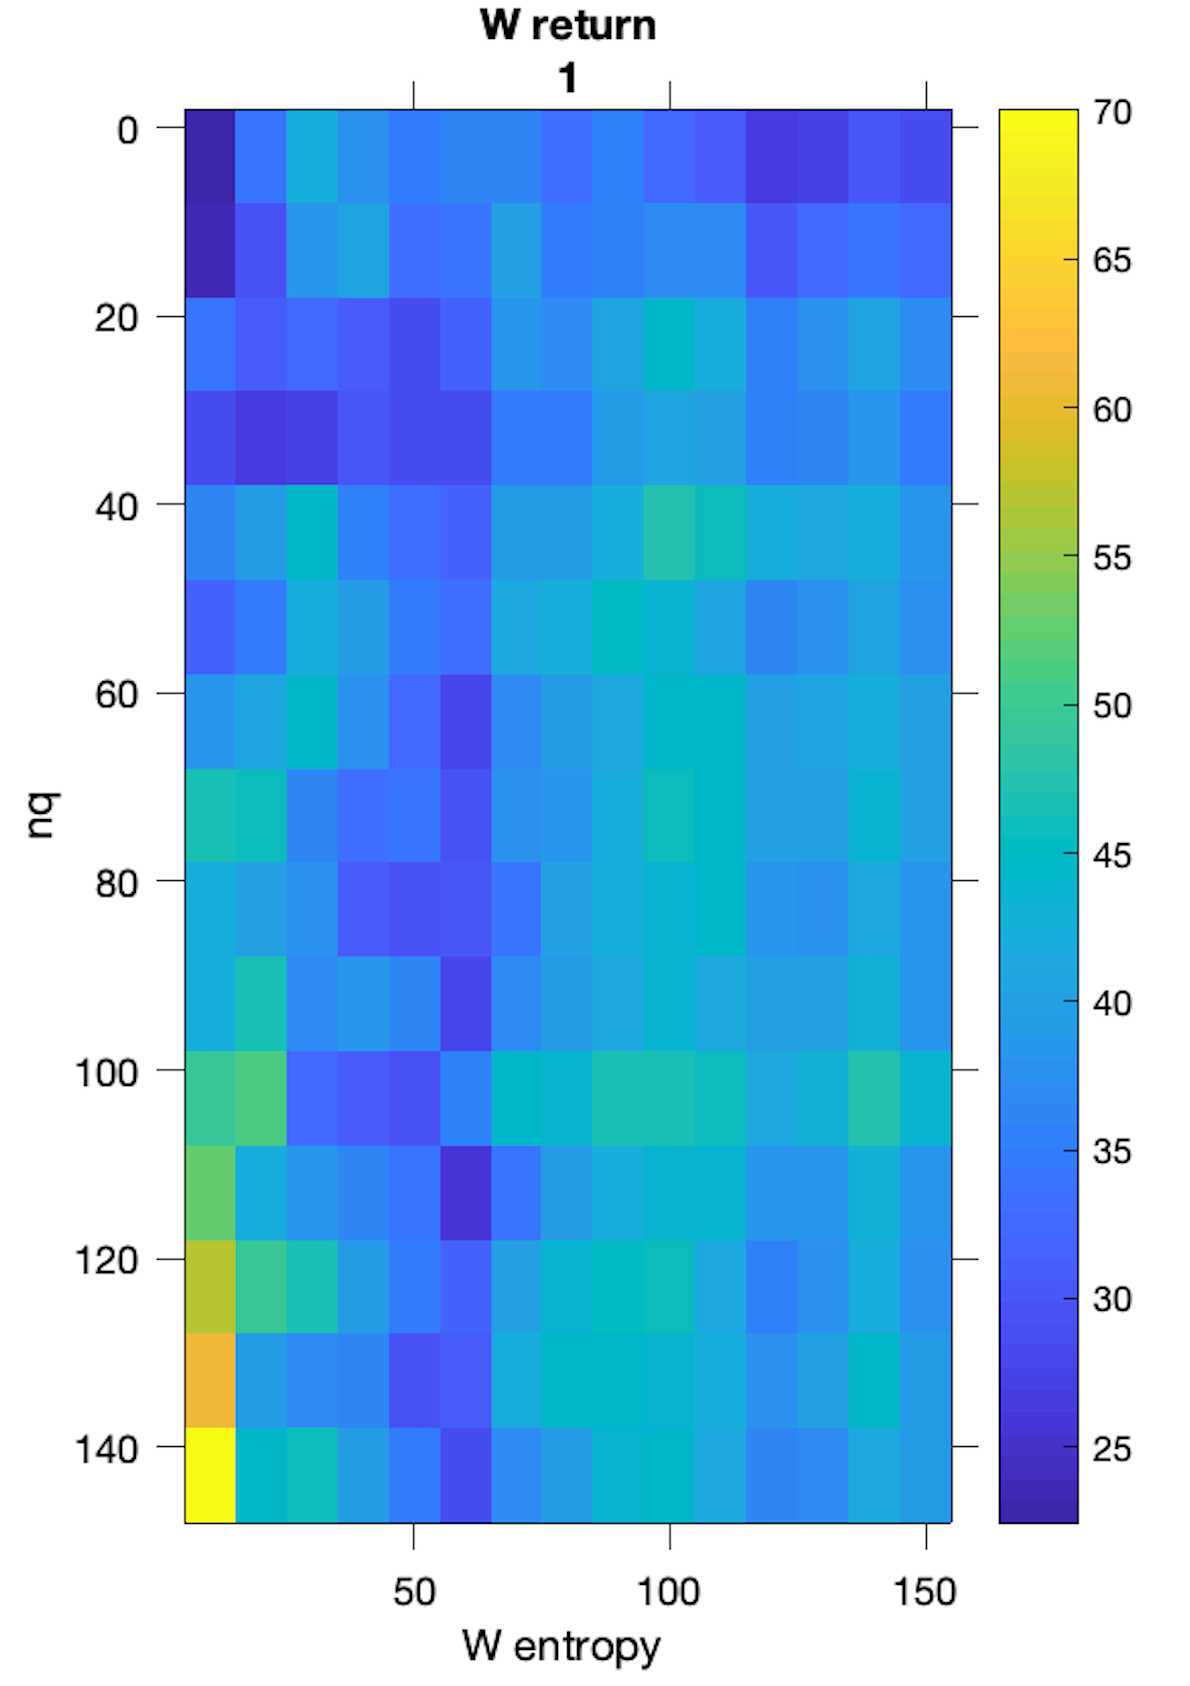
\includegraphics[width=0.7\linewidth]{figures/ejemplo_SNR}
	\caption{Picos que son ruido en el caso de estudio 1 en un "heat map" para la señal a ruido.}
	\label{caso1SNR}
\end{figure}

El caso en cuestión muestra que hay más de 60 y menos de 65 picos que son ruido en la obtención de esos mínimos de entropía (Ver Figura \ref{caso1SNR_individual}). 
\begin{figure}[h!]
	\centering
	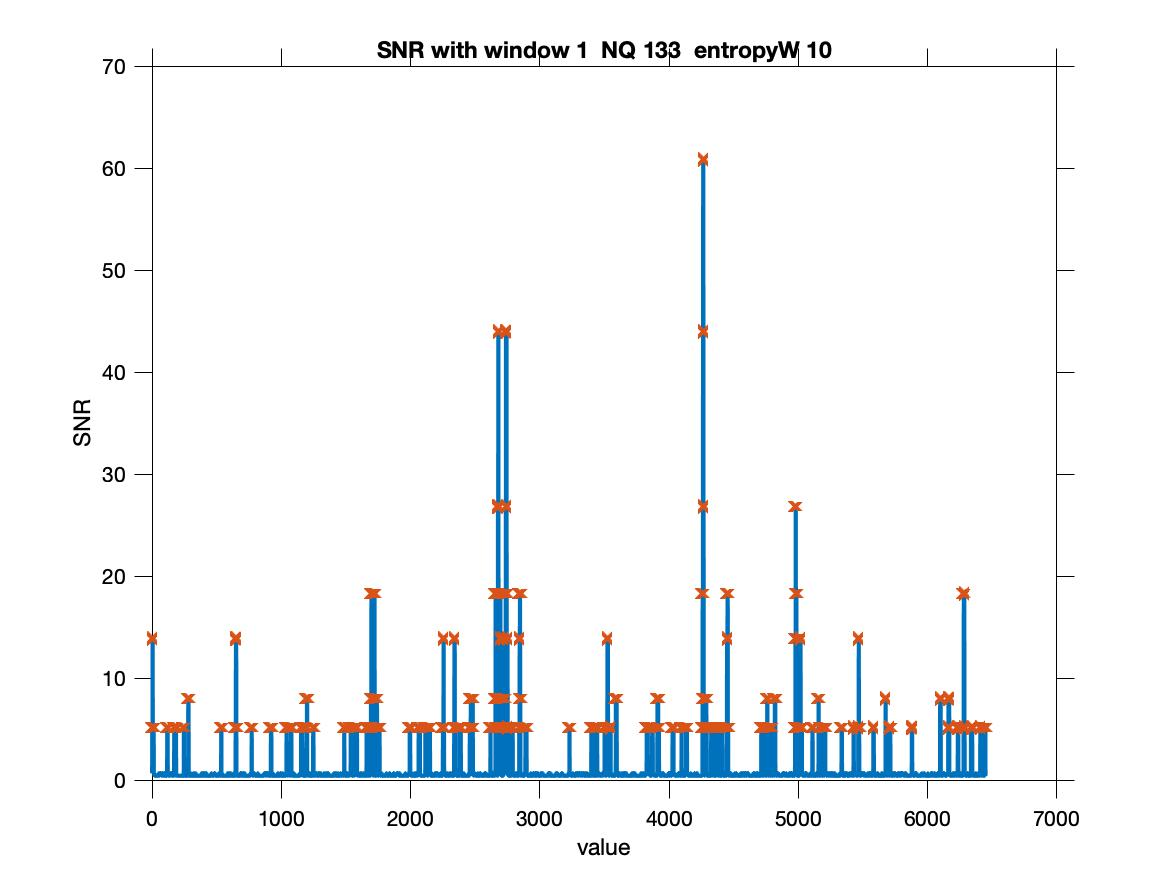
\includegraphics[width=12cm]{figures_matlab/SNR_window_1_NQ_133_entropyW_10.jpg}
	\caption{Señal a ruido para el caso de estudio 1, con una ventana para el cálculo de entropía de 10 en 10 }
	\label{caso1SNR_individual}
\end{figure}


\begin{figure}[h!]
	\centering
	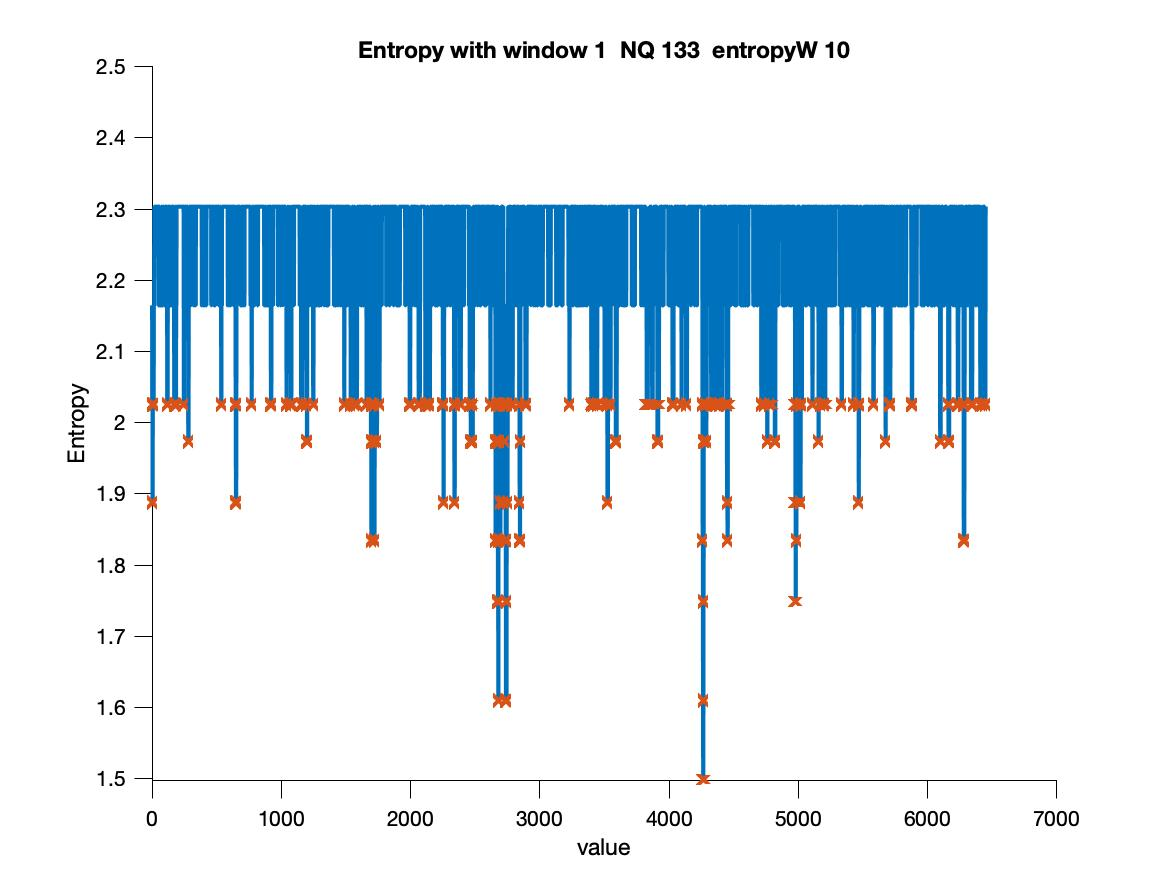
\includegraphics[width=12cm]{figures_matlab/Entropy_window_1_NQ_133_entropyW_10.jpg}
	\caption{Picos que señalan mínimos de entropía para el caso 1, con una ventana para el cálculo de entropía de 10 en 10. }
	\label{caso1entropy_individual}
\end{figure}

Habiendo considerado la señal a ruido los mínimos de entropía para este mismo caso 1 se muestran en la siguiente figura (Ver Figura \ref{caso1entropy_individual}).

\section{Simulación de mercado eficiente}
FALTA EXPLICAR EN METODOLOGIA
Se observan valores mínimos de entropía gracias a la manera en que se presentan los resultados, 
con ello comparar el comportamiento de la entropía del mercado eficiente y del mercado real con fechas, 
con o sin media móvil requiere únicamente del cálculo de un umbral que diferencíe los valores de entropía que se comportan de manera gaussiana  de los que no.


\begin{figure}[h!]
	\centering
	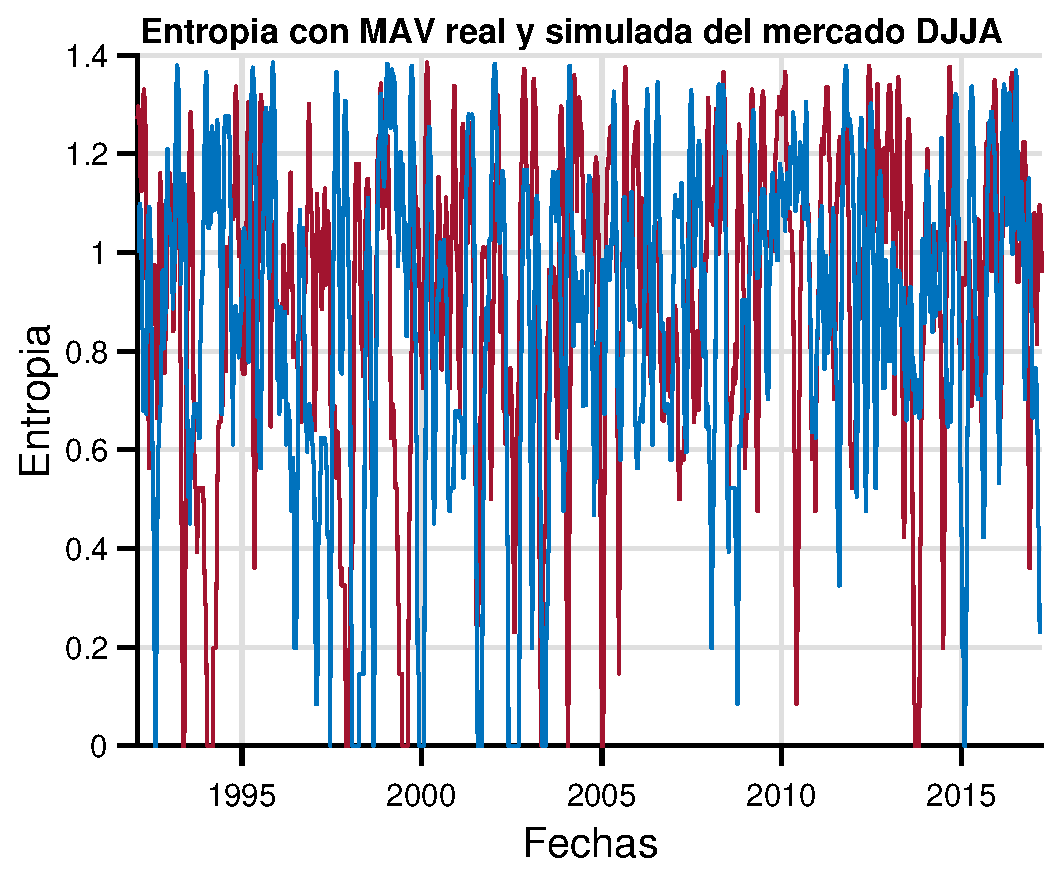
\includegraphics[width=12cm]{figures/MAVentropy}
	\caption{Entropía del mercado real DJJA (línea azul) y un la simulacion de un mercado ideal DJJA (línea roja) con aplicación de medias móviles.}
	\label{fig:maventropy}
\end{figure}

En la gráfica de comparación (Ver figura \ref{fig:maventropy} ) entre la entropía del mercado real y la entropía del mercado simulado se tiene que cuando se simulan los retornos y se les aplica un filtro de media móvil, el cálculo de la entropía muestra que hay mínimos de la entropía con valor cero. Los retornos de datos reales muestran un comportamiento similar ya que hay más de un punto en que la entropía mínima también es cero.


\section{Pruebas estadisticas}

Finalmente, se aplica una prueba estadística de distribuciones a los valores con mínima entropía, tanto de aquellos que fueron tratados con un filtro de media móvil como aquellos que no. 


Recordemos que de la ecuación de la entropía de Shannon se realiza la suma de la probabilidad del estado, multiplicado por la probabilidad del estado. Gracias a que se trabajan con probabilidades es posible graficar un histograma de las entropías, y además se puede estudiar la entropía mediante cuantiles de manera análoga con los retornos de los precios.

Calcular el intervalo de confianza para la distribución de estas entropías sale de este trabajo de tesis, ya que no se asemeja ni a una distribución normal ni a una distribución de Student, ello implicaría tener que realizar interpolaciones entre los cuantiles obtenidos tal como se muestra en el artículo A Method for Confidence Intervals of High Quantiles de Mei Ling Huang, y Xiang Raney-Yan publicado en 2021 \citep[][]{Huang2021}. 
%file:///D:/dark_/descarga_chrome/entropy-23-00070-v3.pdf

Por lo anterior, se propone utilizar como umbral para hallar los valores mínimos de entropía el valor del percentil 95 en vez de un íntervalo de confianza. Por ejemplo, en el mercado DJJA entre el año 2000 y 2005, se aprecia un valor mínimo en el precio, mismo que tiene impacto al estudiar la entropía.


Entonces, al realizar un gráfico que muestra la distribución de la entropía, y dado que la entropía es obtenida a partir de probabilidades, es fácil obtener cualquier cuantil (percentil 95 en el caso del intervalo de confianza), además que dicho percentil permite diferenciar aquellos valores de la entropía que son ruido de aquellos que no. 


\section{Aplicacion del metodo a los mercados NICXFRTRYTKUYLKUTJYRHTEGREF}

